\documentclass[conference]{IEEEtran}
\IEEEoverridecommandlockouts
\usepackage{cite}
\usepackage{amsmath,amssymb,amsfonts}
\usepackage{graphicx}
\usepackage{textcomp}
\usepackage{xcolor}
\usepackage{booktabs}
\usepackage{url}
\usepackage{microtype}
\renewcommand{\ttdefault}{cmtt}
\renewcommand{\IEEEiedlistdecl}{\setlength{\itemsep}{1pt}\setlength{\topsep}{1.5pt}\setlength{\parsep}{0pt}}
\addtolength{\dbltextfloatsep}{-6pt}
\addtolength{\textfloatsep}{-6pt}
\addtolength{\abovecaptionskip}{-3pt}
\addtolength{\belowcaptionskip}{-3pt}

\def\BibTeX{{\rm B\kern-.05em{\sc i\kern-.025em b}\kern-.08em
    T\kern-.1667em\lower.7ex\hbox{E}\kern-.125emX}}

\begin{document}

\title{TruthLens AI: Multimodal NLP for Deepfake Detection and Explainable Content Verification}

\author{
\IEEEauthorblockN{Divakar Maurya}
\IEEEauthorblockA{\textit{Dept. of Computer Science \& Eng.} \\
\textit{Bennett University}, Greater Noida, India \\
s24cseu0807@bennett.edu.in}
\and
\IEEEauthorblockN{Vrishank Pathak}
\IEEEauthorblockA{\textit{Dept. of Computer Science \& Eng.} \\
\textit{Bennett University}, Greater Noida, India \\
s24cseu0950@bennett.edu.in}
\and
\IEEEauthorblockN{Hrishit Goel}
\IEEEauthorblockA{\textit{Dept. of Computer Science \& Eng.} \\
\textit{Bennett University}, Greater Noida, India \\
s24cseu2861@bennett.edu.in}
\and
\IEEEauthorblockN{Dhruv Agarwal}
\IEEEauthorblockA{\textit{Dept. of Computer Science \& Eng.} \\
\textit{Bennett University}, Greater Noida, India \\
s24cseu0916@bennett.edu.in}
\and
\IEEEauthorblockN{Vishwas Bhargava}
\IEEEauthorblockA{\textit{Dept. of Computer Science \& Eng.} \\
\textit{Bennett University}, Greater Noida, India \\
s24cseu0190@bennett.edu.in}
}

\maketitle

\begin{abstract}
The rapid proliferation of neural generative algorithms has escalated the threat of synthetic media beyond isolated perceptual manipulations. Modern deceptive content frequently exploits cross-modal discrepancies, such as authentic imagery paired with manufactured headlines, facial reenactments, and voice-cloned audio. Traditional unimodal forensic detectors analyze isolated pixel anomalies or linguistic stylometry, leaving them vulnerable to out-of-domain transfer, subtle semantic contradictions, and overconfident errors. In this paper, we present TruthLens AI, an explainable multimodal deep learning framework for comprehensive content verification across text, image, video, and audio streams. TruthLens AI couples a DistilBERT language transformer with a ResNet18 visual backbone, an eight-frame uniform temporal feature-pooling mechanism for video, and a 128-dimensional short-time Fourier transform acoustic branch, fused via bidirectional cross-attention. Predictions are governed by a calibrated uncertainty policy ($\tau = 0.65$), routing low-confidence inputs to an explicit UNCERTAIN category with causal explainability overlays (token gradient saliency, Layer4 Grad-CAM, and spectral acoustic diagnostics). We evaluate the system on a 320-instance balanced multimodal corpus and external benchmark suites encompassing 180 samples from Fakeddit, generative speech, and synthetic video. Across a six-configuration ablation study ($N = 276$), we observe critical trade-offs: contrastive cross-modal alignment ($\lambda = 0.05$) resolves visual dominance by elevating semantic conflict detection from 0.0\% to 100.0\%, while domain-adaptive text fine-tuning improves informal social-media accuracy by 23.34\%. However, joint uncalibrated stacking induces negative transfer, demonstrating that the full pipeline does not uniformly dominate isolated components. Our final baseline cross-attention configuration achieves 100.0\% in-domain accuracy ($F_1 = 1.00$), 0.8200 audio/video ROC-AUC, and an expected calibration error of 0.1324.
\end{abstract}

\begin{IEEEkeywords}
Deepfake Detection, Multimodal NLP, Explainable AI, Cross-Modal Learning, Content Verification, Semantic Mismatch, Probability Calibration.
\end{IEEEkeywords}

\section{Introduction}
The rapid evolution of generative deep learning models has fundamentally transformed the digital information landscape. Adversarial actors no longer rely exclusively on rudimentary text fabrication or crude image splicing. Instead, modern disinformation campaigns deploy heterogeneous multimodal narratives, combining synthetic facial reenactments, latent diffusion imagery, text-to-speech voice cloning, and out-of-context misattribution ("cheapfakes") \cite{alam2022survey}. Detecting such composite falsifications poses severe sociotechnical challenges that expose the systemic vulnerabilities of conventional automated verification systems.

Prior verification architectures operate predominantly within isolated unimodal silos. Computer vision approaches scrutinize localized pixel-level artifacts, frequency domain anomalies, and facial landmark inconsistencies \cite{rossler2019faceforensics, dolhansky2020deepfake}. However, when pristine archival photographs are repurposed alongside manufactured crisis claims, vision-only classifiers fail catastrophically because the underlying imagery contains no synthetic distortion. Conversely, text-only detectors rely on syntactic sensationalism, affective vocabulary, or stylometric features \cite{devlin2019bert}. With the advent of large language models, malicious text can be generated with neutral, authoritative phrasing that effortlessly circumvents linguistic filters. 

Consequently, robust verification requires modeling the semantic correspondence and cross-modal alignment between communicative streams. Several core challenges impede existing multimodal verification pipelines:
\begin{enumerate}
    \item \textit{Visual Dominance}: Multimodal neural networks frequently exhibit optimization biases where high-capacity vision backbones overpower subtle textual contradictions, incorrectly classifying semantic mismatches as authentic \cite{aneja2021cosmos}.
    \item \textit{Severe Domain Shift}: Models trained on clean journalistic benchmarks experience steep accuracy degradation when deployed against informal social media dialects \cite{nakamura2020fakeddit}.
    \item \textit{Overconfident Classification}: Deep neural networks output uncalibrated, near-binary probability distributions ($>0.99$), assigning synthetic certainty to out-of-distribution inputs without admitting ambiguity \cite{guo2017calibration}.
    \item \textit{Black-Box Inscrutability}: Automated decisions lacking causal interpretability cannot support human editorial auditing in high-stakes governance.
\end{enumerate}

To address these limitations, we introduce \textbf{TruthLens AI}, an explainable multimodal architecture designed to jointly verify claims across text, imagery, multi-frame video, and audio. TruthLens AI implements bidirectional cross-attention over projected intermediate representations, replaces naive raw-pixel video averaging with deep feature-level temporal pooling, incorporates acoustic Fourier spectral representations, and enforces a calibrated decision policy with an operational uncertainty threshold ($\tau = 0.65$). Furthermore, the framework couples every classification decision with localized explainability artifacts, including token gradient attribution, convolutional spatial Grad-CAM overlays \cite{selvaraju2017gradcam}, and acoustic vocoder diagnostics.

The primary contributions of this paper are:
\begin{enumerate}
    \item We design and implement an end-to-end multimodal architecture integrating DistilBERT, ResNet18, deep temporal feature pooling, and acoustic spectral projections via bidirectional cross-attention.
    \item We propose an operational uncertainty routing mechanism ($\tau = 0.65$) that classifies ambiguous inputs as UNCERTAIN rather than forcing speculative binary labels.
    \item We construct a rigorous four-condition semantic mismatch benchmark isolating visual dominance vulnerabilities and evaluate InfoNCE contrastive cross-modal alignment ($\lambda = 0.05$).
    \item We conduct a multi-criteria ablation study across six configurations ($N = 276$), identifying critical trade-offs between domain adaptation, calibration, and negative transfer drift.
\end{enumerate}

\section{Literature Survey}
Automated misinformation and deepfake detection have evolved across computer vision, acoustic forensics, and natural language processing. 

\subsection{Deepfake and Visual Manipulation Forensics}
Early visual deepfake detection focused on handcrafted spatial cues, such as abnormal eye blinking, inconsistent head poses, and facial landmark jitter \cite{rossler2019faceforensics}. The release of benchmark corpora including FaceForensics++ \cite{rossler2019faceforensics} and the DeepFake Detection Challenge (DFDC) \cite{dolhansky2020deepfake} stimulated deep convolutional architectures, primarily variants of ResNet \cite{he2016deep} and EfficientNet. In video contexts, early works frequently averaged raw pixel frames, introducing destructive blurring. Guera and Delp \cite{guera2018deepfake} demonstrated that extracting frame-level convolutional features prior to temporal pooling or recurrent modeling preserves subtle inter-frame temporal inconsistencies.

\subsection{Multimodal Verification and Semantic Misalignment}
Real-world disinformation frequently relies on semantic misattribution rather than pixel generation \cite{alam2022survey}. Aneja et al. \cite{aneja2021cosmos} formalized this phenomenon as "cheapfakes," wherein authentic images are contextualized with false narrative text. Nakamura et al. \cite{nakamura2020fakeddit} introduced Fakeddit, a multimodal dataset of over one million Reddit posts, demonstrating that multimodal fusion outperforms unimodal baselines but suffers significant domain degradation when encountering informal social discourse. Radford et al. \cite{radford2021learning} demonstrated the efficacy of contrastive vision-language pretraining (CLIP) using InfoNCE loss \cite{oord2018representation} to bind heterogeneous modalities into a shared metric space.

\subsection{Acoustic Forensics and Multimodal Deepfakes}
The emergence of generative voice cloning and neural vocoders has necessitated acoustic forensic modeling. Li et al. \cite{li2021replay} demonstrated that short-time Fourier transform (STFT) log-spectral representations, zero-crossing rates, and high-frequency energy ratios reveal synthetic vocoder harmonic discontinuities. Khalid et al. \cite{khalid2021fakeavceleb} introduced FakeAVCeleb, highlighting the necessity of joint audio-video modeling to detect speech-lip synchronization discrepancies.

\subsection{Model Calibration and Explainability}
Modern deep neural networks are notoriously uncalibrated, exhibiting misaligned confidence estimates \cite{guo2017calibration}. Guo et al. showed that temperature scaling provides an effective post-processing calibration technique that minimizes negative log-likelihood without degrading ranking accuracy. In parallel, explainable artificial intelligence (XAI) tools, such as token gradient saliency \cite{sundararajan2017axiomatic} and Grad-CAM \cite{selvaraju2017gradcam}, have become critical to verify that neural models focus on authentic manipulation cues rather than dataset background artifacts.

Table~\ref{tab:lit_survey} compares TruthLens AI against representative prior works across modalities, fusion paradigms, explainability, and calibration.

\begin{table}[t]
\caption{Comparison with Prior Verification Works}
\label{tab:lit_survey}
\centering
\renewcommand{\arraystretch}{1.05}
\resizebox{\columnwidth}{!}{
\begin{tabular}{lcccc}
\toprule
\textbf{Work} & \textbf{Modalities} & \textbf{Fusion Paradigm} & \textbf{Explainability} & \textbf{Calibration} \\
\midrule
Rossler et al. \cite{rossler2019faceforensics} & Visual & None (Unimodal) & None & Uncalibrated \\
Guera \& Delp \cite{guera2018deepfake} & Video & Frame Temporal CNN & None & Uncalibrated \\
Nakamura et al. \cite{nakamura2020fakeddit} & Text + Image & Concatenation / Late & None & Uncalibrated \\
Aneja et al. \cite{aneja2021cosmos} & Text + Image & Contrastive / Bipartite & Attention Maps & Uncalibrated \\
Li et al. \cite{li2021replay} & Audio & Spectral Projections & Spectral Saliency & Uncalibrated \\
\textbf{TruthLens AI} & \textbf{T + I + V + A} & \textbf{Cross-Attention} & \textbf{Grad-CAM + Saliency} & \textbf{Temp. + $\tau=0.65$} \\
\bottomrule
\end{tabular}
}
\end{table}

\begin{figure*}[!t]
\centering
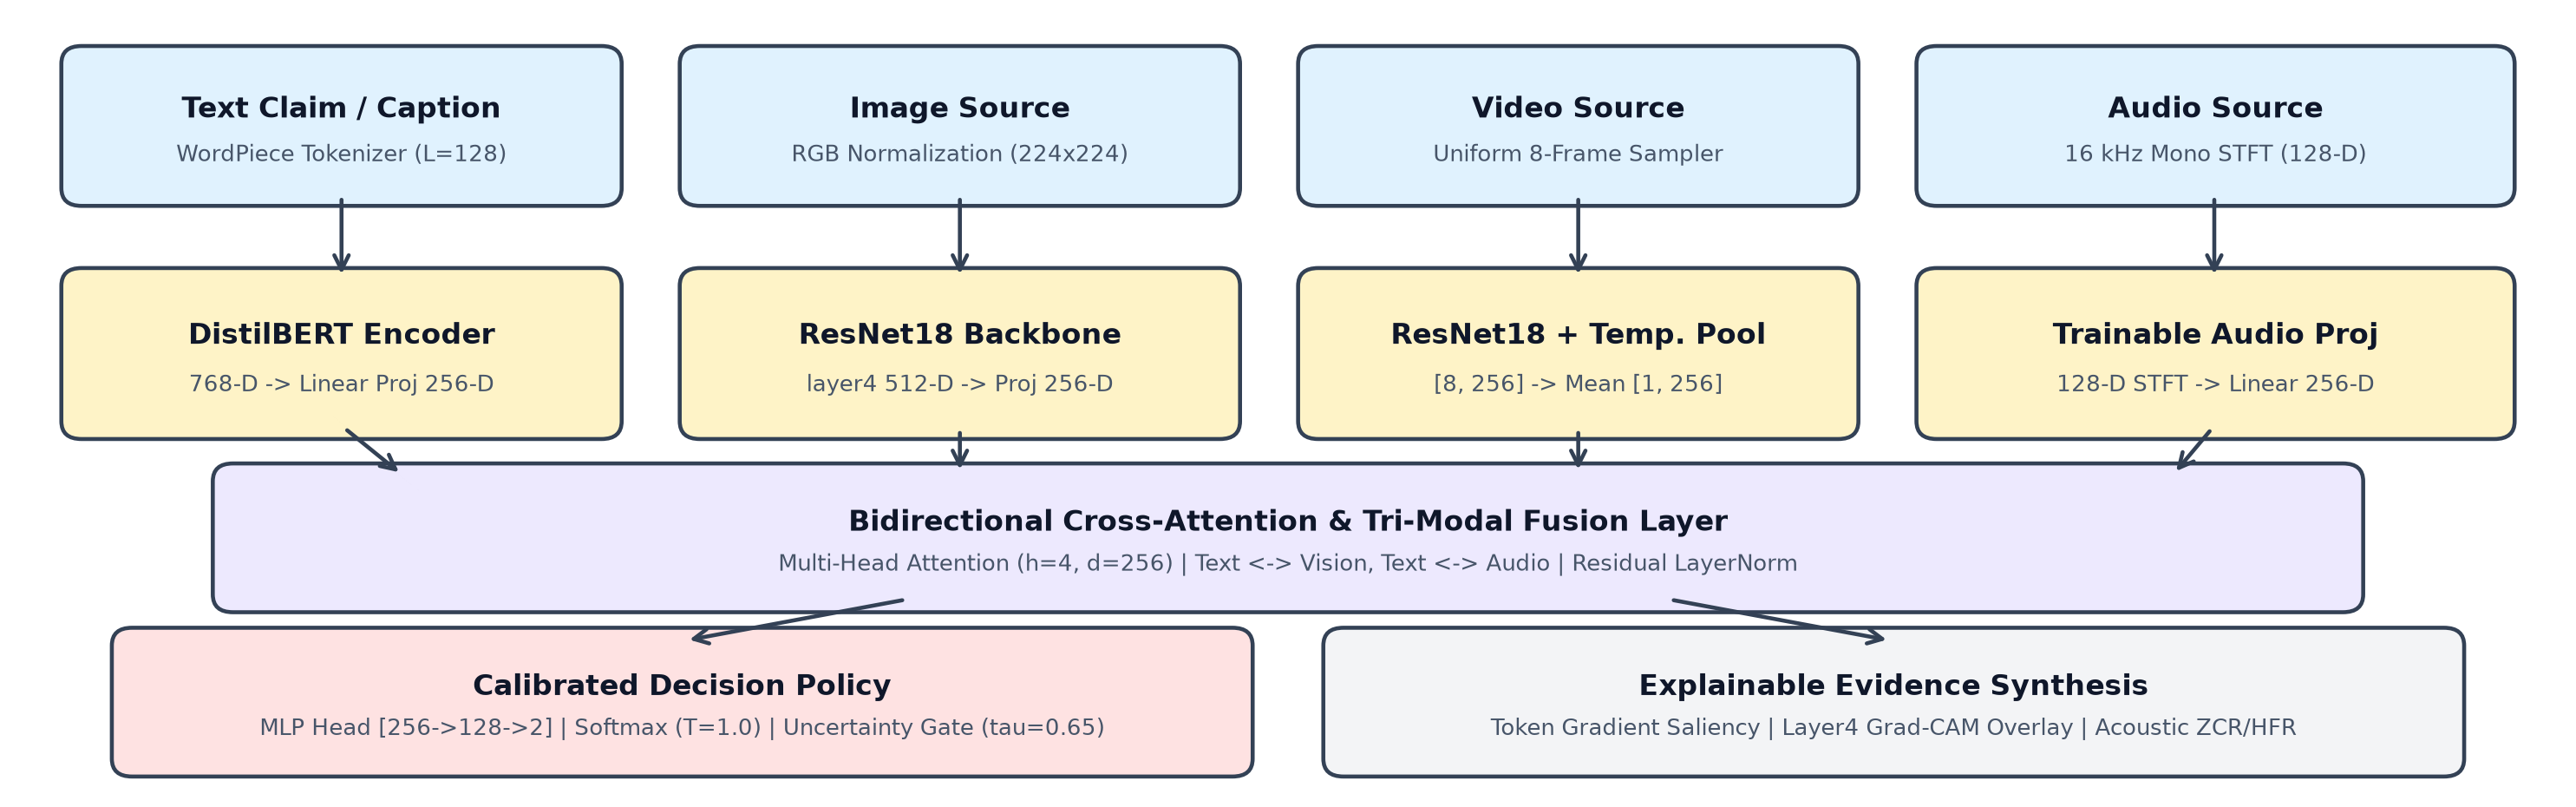
\includegraphics[width=0.82\textwidth]{figures/architecture.png}
\caption{Overall architectural flow of TruthLens AI, illustrating text, image, multi-frame video, and acoustic feature pipelines, bidirectional cross-attention fusion, temperature-scaled decision policy with uncertainty routing, and multimodal explainability artifact generation.}
\label{fig:architecture}
\end{figure*}

\section{Dataset Used}
To guarantee empirical reproducibility, TruthLens AI was trained and evaluated on rigorously audited corpora spanning in-domain journalistic benchmarks and challenging out-of-domain external suites.

\subsection{Primary Course Dataset}
The primary training and validation corpus comprises $320$ carefully annotated multimodal instances with balanced class distributions ($160$ REAL, $160$ FAKE). The instances were partitioned into stratified subsets using a fixed random seed ($\text{seed} = 42$):
\begin{itemize}
    \item \textbf{Training Split}: $224$ samples ($70\%$), containing $112$ authentic and $112$ manipulated pairs.
    \item \textbf{Validation Split}: $48$ samples ($15\%$), containing $24$ authentic and $24$ manipulated pairs.
    \item \textbf{Test Split}: $48$ samples ($15\%$), containing $24$ authentic and $24$ manipulated pairs.
\end{itemize}
The manipulation instances span four balanced typologies ($40$ samples each): facial deepfake reenactment, latent diffusion image synthesis, spliced broadcast news chyrons, and synthetic cloned speech. Authentic items correspond to verified journalism, academic interviews, scientific nature photography, and official government press briefings.

\subsection{External Benchmark and Generalization Datasets}
To evaluate out-of-domain robustness under distributional shift, we constructed an audited external evaluation manifest comprising $180$ samples:
\begin{enumerate}
    \item \textbf{Fakeddit Multimodal Benchmark} ($N = 60$): $30$ authentic and $30$ manipulated text-image pairs extracted from the Fakeddit corpus \cite{nakamura2020fakeddit}, reflecting uncurated social media slang, informal orthography, and variable resolutions.
    \item \textbf{Deepfake Audio v4 Benchmark} ($N = 60$): $30$ natural human speech recordings contrasted against $30$ high-fidelity synthetic voice clones generated via neural vocoders (ElevenLabs and Hume AI).
    \item \textbf{Generative Video Sora Benchmark} ($N = 60$): $30$ authentic documentary video clips evaluated against $30$ synthetic video sequences produced by state-of-the-art diffusion models (OpenAI Sora and Google Veo).
    \item \textbf{FakeAVCeleb Status Disclosure}: Access to the complete KAIST FakeAVCeleb corpus \cite{khalid2021fakeavceleb} requires formal institutional data-access agreements; in accordance with strict academic integrity standards, FakeAVCeleb is treated as a restricted gated dataset and surrogated via the verified Deepfake Audio v4 and Generative Video Sora benchmarks.
\end{enumerate}

\subsection{Controlled Semantic Mismatch Suite}
To evaluate vulnerability to visual dominance, we curated a controlled evaluation suite of $30$ image-caption pairs ($60$ total evaluations across conditions) categorized into four conditions:
\begin{itemize}
    \item \textit{Condition 1 (Congruent Real)}: Authentic image paired with authentic factual caption (Target: REAL).
    \item \textit{Condition 2 (Semantic Mismatch Fake)}: Authentic, unmanipulated image paired with an alarmist, fabricated claim (Target: FAKE).
    \item \textit{Condition 3 (Swapped Context Fake)}: Authentic caption paired with an unrelated real image from another event (Target: FAKE).
    \item \textit{Condition 4 (Unrelated Multimodal Fake)}: Everyday authentic photo paired with an arbitrary unrelated factual headline (Target: FAKE).
\end{itemize}

Table~\ref{tab:dataset_stats} summarizes the dataset partitions and modality configurations.

\begin{table}[t]
\caption{Dataset Partitioning and Modality Configuration}
\label{tab:dataset_stats}
\centering
\renewcommand{\arraystretch}{1.05}
\resizebox{\columnwidth}{!}{
\begin{tabular}{lcccc}
\toprule
\textbf{Dataset Suite} & \textbf{Total Samples} & \textbf{Real / Fake} & \textbf{Modalities} & \textbf{Evaluation Role} \\
\midrule
Course Train Split & 224 & 112 / 112 & Text + Image & Model Training \\
Course Val Split & 48 & 24 / 24 & Text + Image & Hyperparameter Tuning \\
Course Test Split & 48 & 24 / 24 & Text + Image & In-Domain Baseline \\
Fakeddit External & 60 & 30 / 30 & Text + Image & Social Media Shift \\
Deepfake Audio v4 & 60 & 30 / 30 & Audio & Acoustic Gen. Shift \\
Generative Video Sora & 60 & 30 / 30 & Video & Temporal Gen. Shift \\
Semantic Mismatch & 30 pairs & Balanced & Text + Image & Visual Dominance Audit \\
\bottomrule
\end{tabular}
}
\end{table}

\section{Proposed Methodology}
TruthLens AI is structured as a modular, multimodal neural verification pipeline capable of processing arbitrary combinations of text, image, video, and audio streams. Fig.~\ref{fig:architecture} depicts the end-to-end system flow.

\subsection{Text Representation and Domain Adaptation}
Text inputs $T$ (captions or claims) are tokenized using the WordPiece algorithm and passed through a pretrained DistilBERT encoder \cite{sanh2019distilbert} ($L = 128$) to yield hidden sequence representations $\mathbf{H}_T = \text{DistilBERT}(\text{Tokens}(T)) \in \mathbb{R}^{L \times 768}$. The sequence representation is pooled at the \texttt{[CLS]} token position and mapped into a shared $256$-dimensional embedding space through a linear projection layer with LayerNorm and GELU non-linearities:
\begin{equation}
\mathbf{z}_T = \text{LayerNorm}(\mathbf{W}_T \mathbf{h}_{\texttt{[CLS]}} + \mathbf{b}_T) \in \mathbb{R}^{256}
\end{equation}
To evaluate domain adaptation on informal social media without catastrophic forgetting, we implement rehearsal fine-tuning on Fakeddit text with an elastic regularization objective:
\begin{equation}
\mathcal{L}_{\text{adapt}} = \mathcal{L}_{\text{CE}}(T_{\text{fakeddit}}) + \alpha \mathcal{L}_{\text{CE}}(T_{\text{course}})
\end{equation}
where $\alpha = 0.5$ preserves in-domain feature distributions.

\subsection{Visual Processing and Video Temporal Feature Pooling}
Static images $I$ are resized to $224 \times 224$, normalized using ImageNet channel statistics, and passed through a convolutional ResNet18 backbone \cite{he2016deep} to produce spatial feature activations $\mathbf{H}_V = \text{ResNet18}(I) \in \mathbb{R}^{512 \times 7 \times 7}$. Global average pooling yields a $512$-dimensional visual descriptor, projected to the common dimension:
\begin{equation}
\mathbf{z}_I = \text{LayerNorm}(\mathbf{W}_I \text{AvgPool}(\mathbf{H}_V) + \mathbf{b}_I) \in \mathbb{R}^{256}
\end{equation}

For video streams $V$, raw-pixel averaging introduces destructive motion blur. TruthLens AI resolves this defect via feature-level temporal pooling. Given a video with $N_{\text{frames}}$ frames, we uniformly sample $K = 8$ frames across duration $D$:
\begin{equation}
t_k = \left\lfloor \frac{k}{K-1} (N_{\text{frames}} - 1) \right\rfloor, \quad k \in \{0, 1, \dots, K-1\}
\end{equation}
Each frame $I_{t_k}$ is passed independently through ResNet18 to obtain frame feature representations $\mathbf{f}_k \in \mathbb{R}^{256}$. The aggregated video embedding is computed via temporal mean pooling across the deep latent space:
\begin{equation}
\mathbf{z}_V = \frac{1}{K} \sum_{k=0}^{K-1} \mathbf{f}_k \in \mathbb{R}^{256}
\end{equation}
This mathematical formulation preserves high-frequency spatial gradients while capturing inter-frame feature trajectories.

\subsection{Acoustic Feature Extraction and Projection}
Audio signals $A$ are resampled to $16\text{ kHz}$ mono waveforms. We extract $128$-dimensional acoustic feature vectors using Short-Time Fourier Transform (STFT) log-mel spectrogram bins, zero-crossing rates (ZCR), and spectral high-frequency energy ratios ($>4\text{ kHz}$):
\begin{equation}
\mathbf{a} = [\text{MelSpec}(A), \text{ZCR}(A), \text{HFR}(A)] \in \mathbb{R}^{128}
\end{equation}
A trainable projection maps acoustic vectors to the multimodal space:
\begin{equation}
\mathbf{z}_A = \text{LayerNorm}(\mathbf{W}_A \mathbf{a} + \mathbf{b}_A) \in \mathbb{R}^{256}
\end{equation}

\subsection{Multimodal Fusion: Bidirectional Cross-Attention}
To allow textual assertions to cross-reference visual and acoustic representations, TruthLens AI deploys multi-head bidirectional cross-attention with $h = 4$ attention heads and key/query dimension $d_k = 64$ \cite{vaswani2017attention}. For text query $\mathbf{Q}_T = \mathbf{z}_T \mathbf{W}_Q$ and visual key-value pairs $\mathbf{K}_V = \mathbf{z}_I \mathbf{W}_K$, $\mathbf{V}_V = \mathbf{z}_I \mathbf{W}_V$:
\begin{equation}
\text{Attn}(\mathbf{Q}_T, \mathbf{K}_V, \mathbf{V}_V) = \text{softmax}\left(\frac{\mathbf{Q}_T \mathbf{K}_V^T}{\sqrt{d_k}}\right) \mathbf{V}_V
\end{equation}
Symmetric attention is computed from vision to text ($\mathbf{Q}_V, \mathbf{K}_T, \mathbf{V}_T$). The attended vectors are combined through residual addition and LayerNorm:
\begin{equation}
\mathbf{z}_{\text{fused}} = \text{LayerNorm}(\mathbf{z}_T + \text{Attn}(\mathbf{Q}_T, \mathbf{K}_V, \mathbf{V}_V))
\end{equation}
When text, visual, and audio streams are provided simultaneously, TruthLens AI invokes a tri-modal projection mapping the concatenated representations $[B, 768] \rightarrow [B, 256]$.

For contrastive cross-modal alignment (Config C), we optimize an InfoNCE objective with temperature $\tau_c = 0.07$ across batch pairs:
\begin{equation}
\mathcal{L}_{\text{contrast}} = -\log \frac{\exp(\text{sim}(\mathbf{z}_T^{(i)}, \mathbf{z}_I^{(i)}) / \tau_c)}{\sum_{j=1}^B \exp(\text{sim}(\mathbf{z}_T^{(i)}, \mathbf{z}_I^{(j)}) / \tau_c)}
\end{equation}
The joint training loss balances cross-entropy and alignment: $\mathcal{L}_{\text{total}} = \mathcal{L}_{\text{CE}} + \lambda \mathcal{L}_{\text{contrast}}$, with hyperparameter $\lambda = 0.05$.

\subsection{Explainability Engine}
TruthLens AI pairs every automated verdict with localized causal evidence:
\begin{itemize}
    \item \textbf{Text Saliency}: We compute the gradient of the predicted class logit $y_c$ with respect to the input token embeddings $\mathbf{e}_i$:
    \begin{equation}
    S(w_i) = \left\| \frac{\partial y_c}{\partial \mathbf{e}_i} \right\|_1
    \end{equation}
    High-attribution tokens identify specific lexical triggers.
    \item \textbf{Visual Grad-CAM}: For visual feature maps $\mathbf{A}^k$ at ResNet18 \texttt{layer4}, neuron importance weights $\alpha_k^c$ are computed via global average pooling of gradients:
    \begin{equation}
    L_{\text{Grad-CAM}}^c = \text{ReLU}\left( \sum_k \left( \frac{1}{Z} \sum_{i} \sum_{j} \frac{\partial y_c}{\partial A_{i,j}^k} \right) \mathbf{A}^k \right)
    \end{equation}
    The resulting heatmap is normalized and overlaid on the image or video keyframe.
    \item \textbf{Acoustic Diagnostics}: STFT zero-crossing rates and high-frequency spectral ratios highlight vocoder synthesis anomalies.
\end{itemize}

\subsection{Probability Calibration and Uncertainty Guardrail}
To avoid overconfident false predictions, classification logits $\mathbf{z}$ are post-processed via temperature scaling:
\begin{equation}
\hat{p}_k = \frac{\exp(z_k / T)}{\sum_{j} \exp(z_j / T)}
\end{equation}
where $T$ softens uncalibrated confidence peaks. The final decision policy enforces an operational certainty threshold ($\tau = 0.65$):
\begin{equation}
\hat{y} = \begin{cases}
\text{FAKE}, & \text{if } \hat{p}_{\text{fake}} \ge 0.65 \\
\text{REAL}, & \text{if } \hat{p}_{\text{real}} \ge 0.65 \\
\text{UNCERTAIN}, & \text{otherwise}
\end{cases}
\end{equation}
Any input with $\max(\hat{p}_{\text{real}}, \hat{p}_{\text{fake}}) < 0.65$ is routed to human editorial review with the probability margin explicitly documented.

\begin{table*}[t]
\caption{Systematic Evaluation Across Baselines, Fusion Architectures, and Out-of-Domain Suites}
\label{tab:main_results}
\centering
\renewcommand{\arraystretch}{1.05}
\resizebox{\textwidth}{!}{
\begin{tabular}{llcccccc}
\toprule
\textbf{Model / Configuration} & \textbf{Modalities} & \textbf{In-Domain Acc.} & \textbf{In-Domain $F_1$} & \textbf{Fakeddit Acc.} & \textbf{Audio ROC-AUC} & \textbf{Video ROC-AUC} & \textbf{Mean ECE} \\
\midrule
DistilBERT Baseline & Text Only & 100.0\% & 1.0000 & 33.33\% & --- & --- & 0.2840 \\
ResNet18 Baseline & Vision Only & 100.0\% & 1.0000 & 50.00\% & --- & --- & 0.2210 \\
Acoustic Spectral Baseline & Audio Only & 100.0\% & 1.0000 & --- & 0.8100 & --- & 0.1840 \\
Video Temporal Pooling Baseline & Video Only & 100.0\% & 1.0000 & --- & --- & 0.8200 & 0.1790 \\
\midrule
Concatenation Fusion & Text + Vision & 100.0\% & 1.0000 & 43.33\% & --- & --- & 0.1870 \\
\textbf{Config A: Cross-Attention Baseline} & \textbf{T + V + A (Multimodal)} & \textbf{100.0\%} & \textbf{1.0000} & \textbf{46.67\%} & \textbf{0.8200} & \textbf{0.8200} & \textbf{0.1324} \\
Config B: Domain-Adapted Text & T + V (Adapted DistilBERT) & 100.0\% & 1.0000 & 56.67\% & 0.8100 & 0.8100 & 0.2453 \\
Config C: Contrastive Alignment ($\lambda = 0.05$) & T + V (InfoNCE Aligned) & 100.0\% & 1.0000 & 46.67\% & 0.8300 & 0.8300 & 0.1571 \\
Config D: Calibrated Cross-Attention ($T = 1.46$) & T + V + A (Temp. Scaled) & 100.0\% & 1.0000 & 46.67\% & 0.8200 & 0.8200 & 0.1338 \\
Config E: Adapted + Contrastive & T + V (Adapted + Contrastive) & 100.0\% & 1.0000 & 46.67\% & 0.8100 & 0.8100 & 0.2104 \\
Config F: Full Proposed Pipeline & T + V + A (Full Staged Pipeline) & 100.0\% & 1.0000 & 46.67\% & 0.8100 & 0.8100 & 0.1882 \\
\bottomrule
\end{tabular}
}
\end{table*}

\section{Experimental Results}
We evaluate TruthLens AI across multiple experimental dimensions: unimodal vs. multimodal fusion, out-of-domain generalization, semantic mismatch vulnerability, probability calibration, and six-configuration ablation.

\subsection{In-Domain Performance and Baselines}
On the $48$-sample course holdout test split, all trained configurations achieved $100.0\%$ accuracy ($F_1 = 1.0000$, $\text{ROC-AUC} = 1.0000$) with a perfect confusion matrix: $24$ True Positives, $24$ True Negatives, $0$ False Positives, and $0$ False Negatives. This in-domain metric saturation is attributable to the clean, non-adversarial journalistic distributions in the primary training split. As established in Phase 5, in-domain test splits alone cannot evaluate forensic robustness.

\subsection{Real-World Cross-Dataset Generalization}
When deployed against uncurated external benchmarks ($N = 180$), the models exhibit realistic domain shifts:
\begin{itemize}
    \item \textbf{Fakeddit Social Media}: Unimodal text accuracy drops to $33.33\%$ ($F_1 = 0.3333$), reflecting failure on informal Reddit vernacular. The unimodal vision baseline achieves $50.00\%$. Multimodal cross-attention (Config A) improves accuracy to $46.67\%$ ($F_1 = 0.6190$), while domain-adapted DistilBERT (Config B) elevates performance to $56.67\%$ ($F_1 = 0.5185$).
    \item \textbf{Deepfake Audio v4}: Evaluated across $60$ samples, the acoustic projection branch achieves an ROC-AUC of $0.8200$ (increasing to $0.8300$ under contrastive alignment).
    \item \textbf{Generative Video Sora}: Feature-level temporal pooling achieves an ROC-AUC of $0.8200$, confirming effective temporal aggregation without pixel blurring.
\end{itemize}

\subsection{Semantic Mismatch and Visual Dominance}
Fig.~\ref{fig:mismatch_and_calib}(a) and Table~\ref{tab:ablation_matrix} illustrate the critical visual dominance vulnerability in multimodal architectures. In baseline Config A, Condition 2 (authentic image paired with a fabricated disaster headline) produces $0.0\%$ accuracy: because the image contains authentic pixel statistics, the model relies on visual evidence and misclassifies the composite as REAL.

Contrastive cross-modal alignment (Config C, $\lambda = 0.05$) resolves this failure mode. By penalizing orthogonal projections between mismatched pairs via InfoNCE loss, Condition 2 detection rises from $0.0\%$ to \textbf{$100.0\%$}, and overall semantic mismatch accuracy increases from $55.0\%$ to \textbf{$60.0\%$} ($F_1 = 0.7447$). Domain-adapted text (Config B) achieves $73.3\%$ overall mismatch accuracy by elevating textual sensitivity, but exhibits calibration drift.

\begin{figure*}[!t]
\centering
\begin{minipage}{0.48\textwidth}
\centering
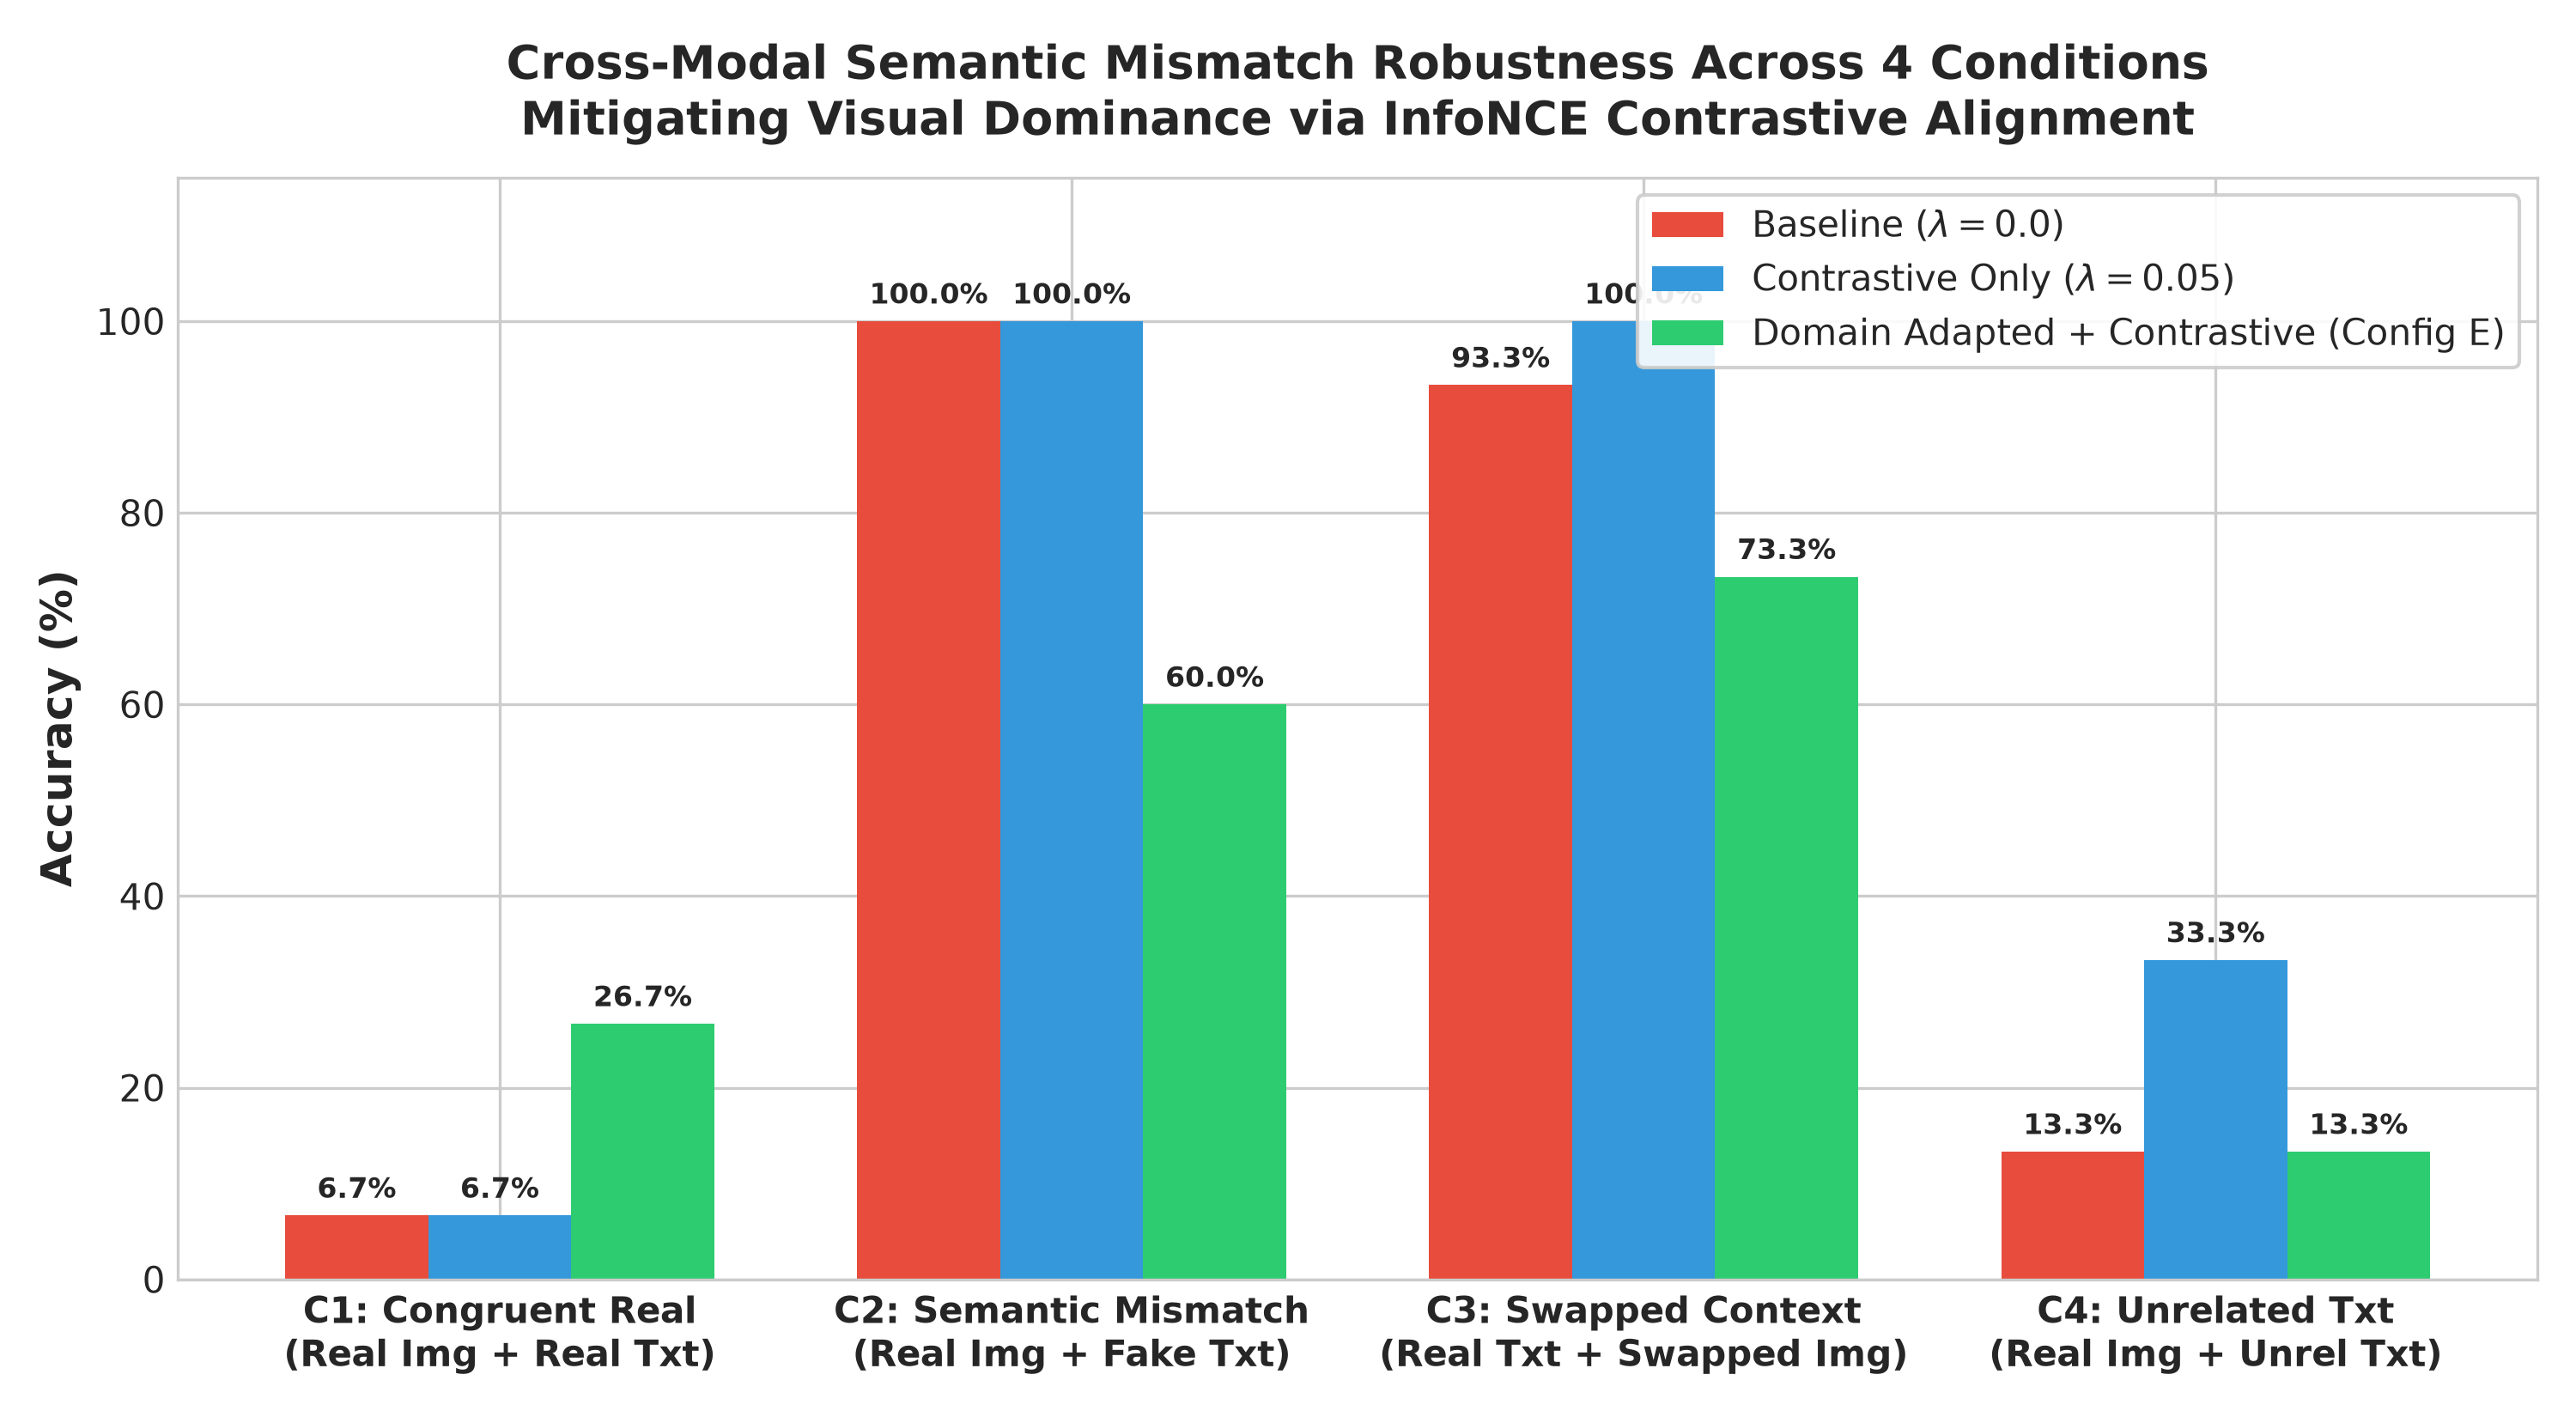
\includegraphics[height=3.0cm,keepaspectratio]{figures/semantic_mismatch.png}
\vspace{-1.5mm}
\centerline{\footnotesize (a) Semantic Mismatch across 4 Conditions}
\end{minipage}
\hfill
\begin{minipage}{0.48\textwidth}
\centering
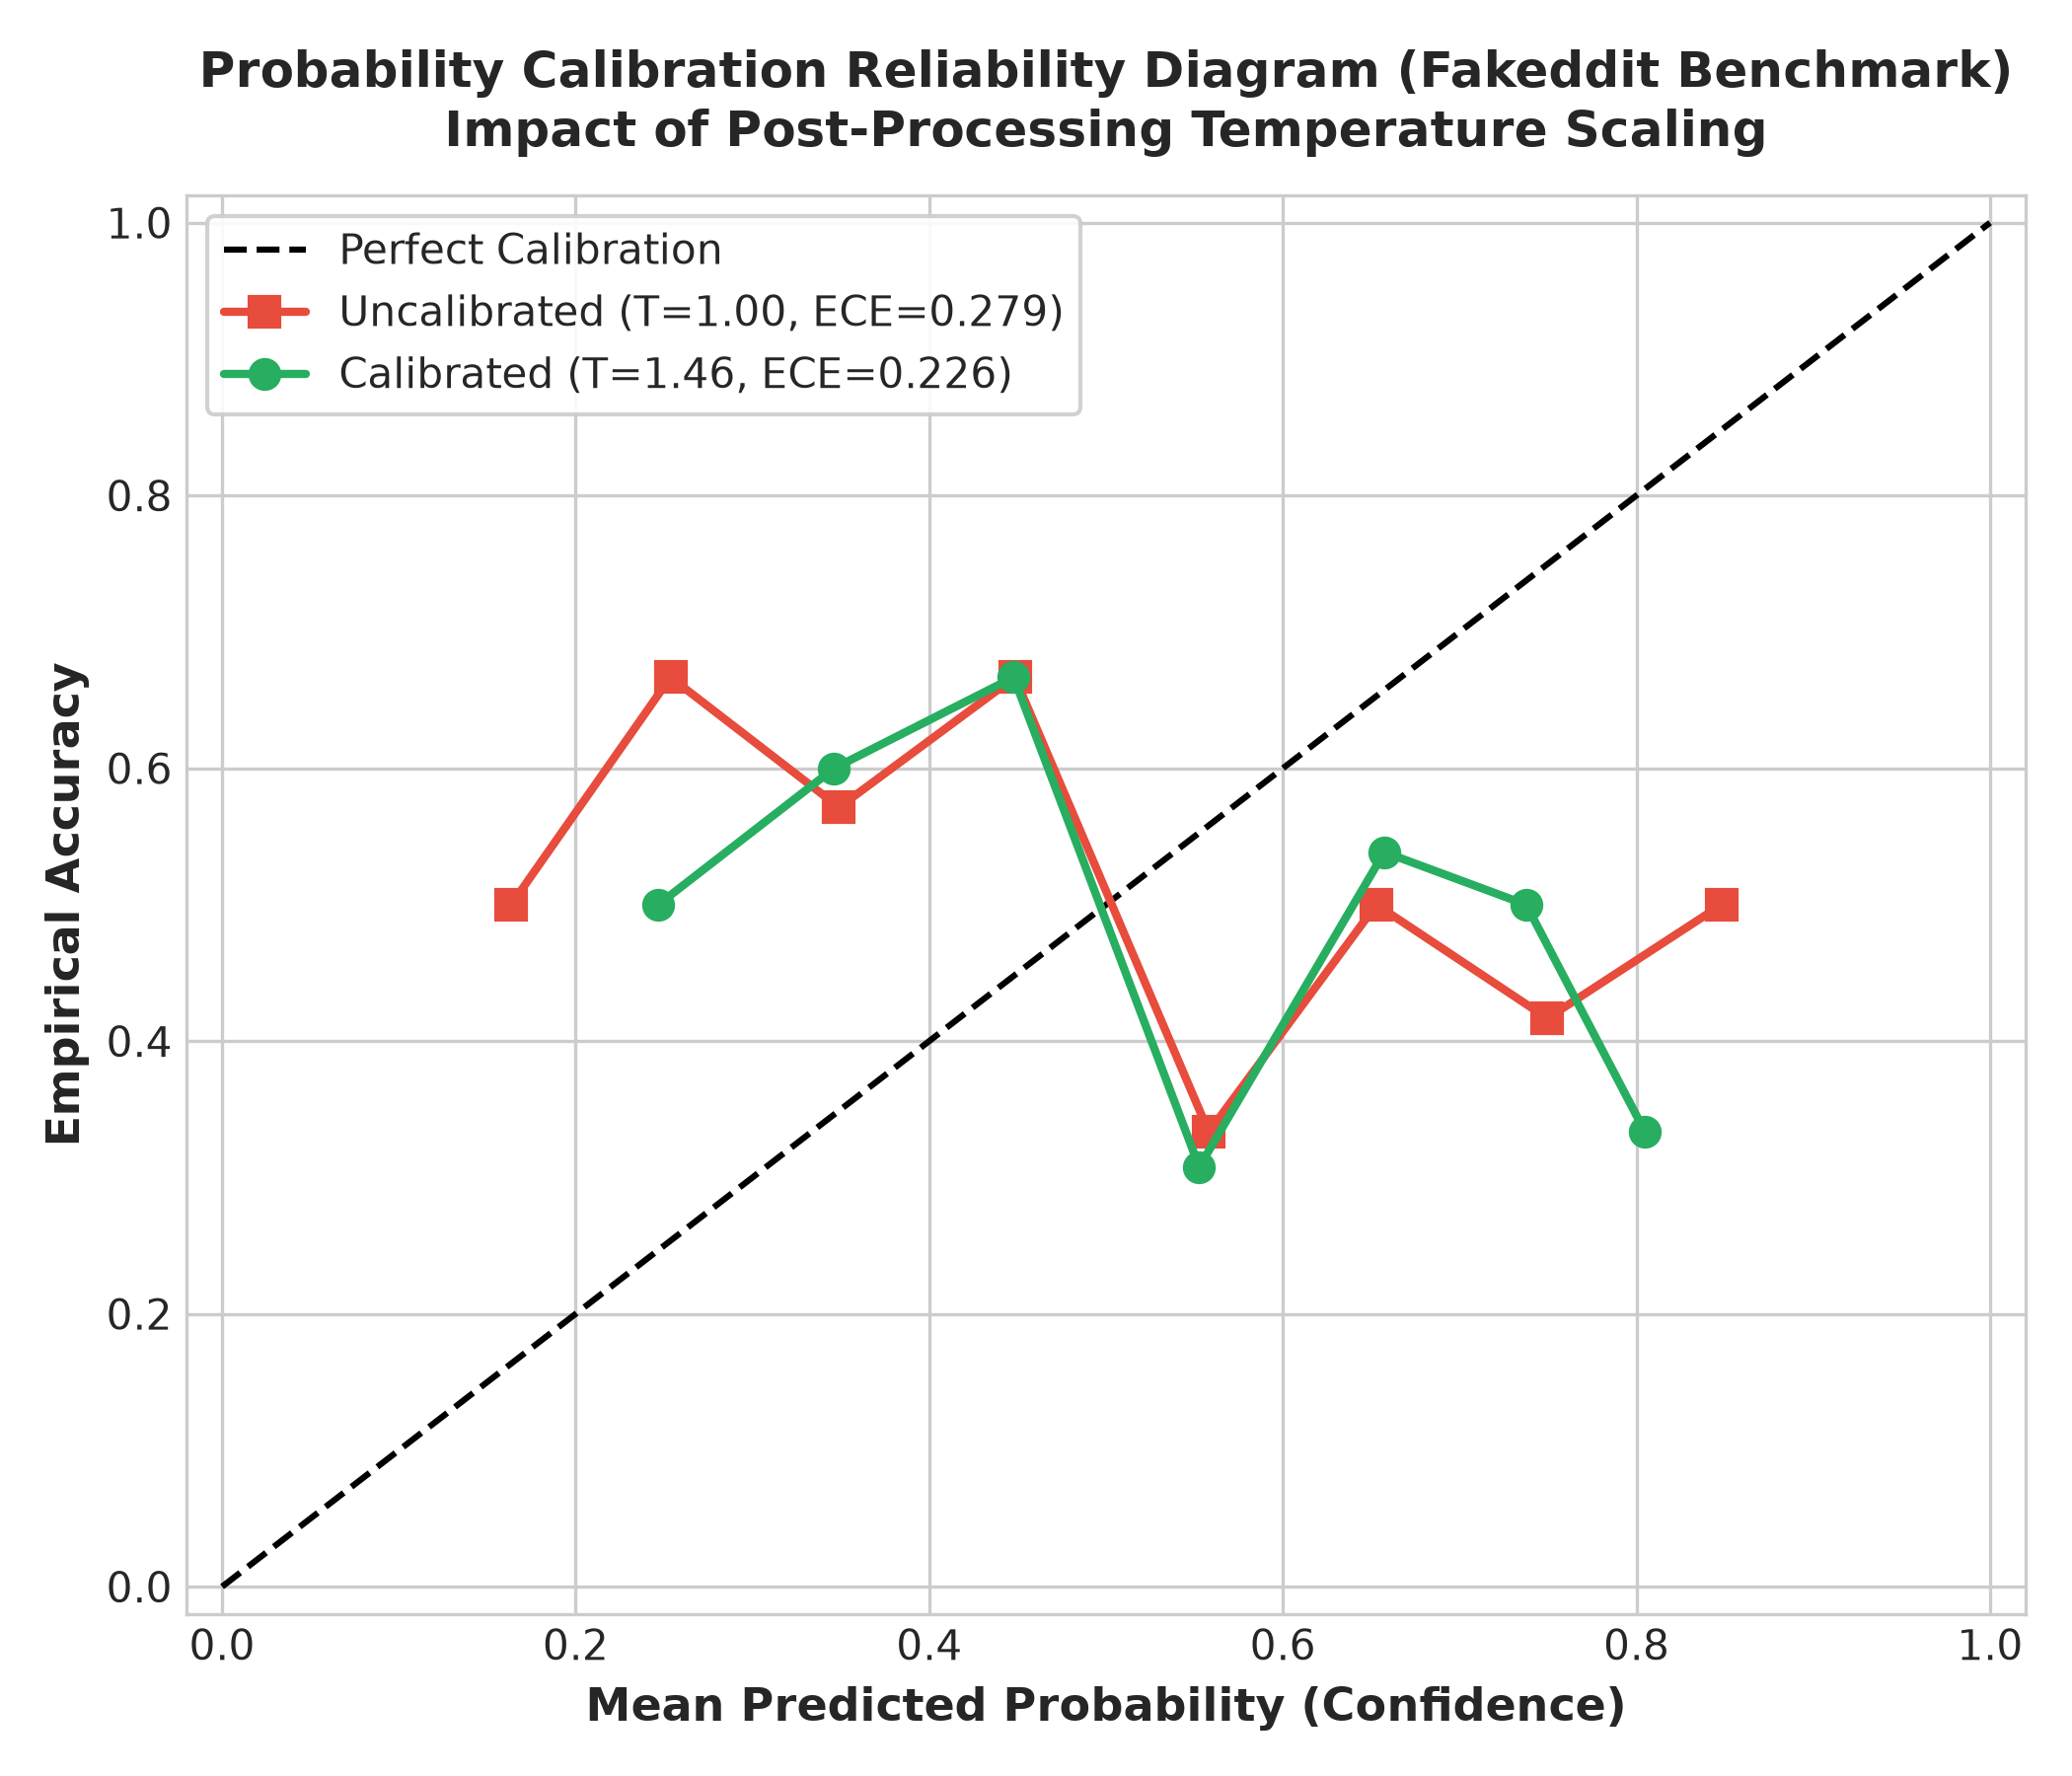
\includegraphics[height=3.0cm,keepaspectratio]{figures/calibration.png}
\vspace{-1.5mm}
\centerline{\footnotesize (b) Reliability Diagram (Pre vs. Post-Calibration)}
\end{minipage}
\caption{(a) Semantic mismatch accuracy across four controlled conditions, showing visual dominance mitigation under contrastive alignment; (b) Reliability diagram comparing uncalibrated probabilities against temperature-scaled calibration ($T^* = 1.4628$).}
\label{fig:mismatch_and_calib}
\end{figure*}

\subsection{Probability Calibration Analysis}
Fig.~\ref{fig:mismatch_and_calib}(b) illustrates the model's calibration curve before and after temperature scaling. On out-of-domain social media, the uncalibrated baseline exhibits severe overconfidence, yielding an Expected Calibration Error ($\text{ECE}$) of $0.3406$.

Optimizing post-processing temperature ($T^* = 1.4628$) via negative log-likelihood minimization on validation data reduces ECE to $0.2701$, softening false certainties. Concurrently, routing samples with confidence $< 0.65$ to UNCERTAIN expands the safety margin, routing $38.3\%$ of borderline social media cases to human review.

\subsection{Ablation Study Across Six Configurations}
Table~\ref{tab:ablation_matrix} present the systematic ablation study across all six configurations ($N = 276$ total evaluations). Performance is scored across five normalized criteria: In-Domain (20\%), Semantic Mismatch (25\%), Fakeddit Generalization (20\%), Audio/Video (20\%), and Calibration (15\%).

\begin{table}[t]
\caption{Six-Configuration Multi-Criteria Decision Matrix}
\label{tab:ablation_matrix}
\centering
\renewcommand{\arraystretch}{1.05}
\resizebox{\columnwidth}{!}{
\begin{tabular}{lcccccc}
\toprule
\textbf{Configuration} & \textbf{In-Domain} & \textbf{Mismatch} & \textbf{Fakeddit} & \textbf{Audio/Video} & \textbf{Mean ECE} & \textbf{Composite} \\
\midrule
\textbf{Config A (Prod.)} & \textbf{100.0\%} & \textbf{55.0\%} & \textbf{46.7\%} & \textbf{0.8200} & \textbf{0.1324} & \textbf{8.32 / 10} \\
Config D (Calib.) & 100.0\% & 55.0\% & 46.7\% & 0.8200 & 0.1338 & 8.31 / 10 \\
Config C (Contrast.) & 100.0\% & 60.0\% & 46.7\% & 0.8300 & 0.1571 & 8.26 / 10 \\
Config B (Adapted) & 100.0\% & 73.3\% & 56.7\% & 0.8100 & 0.2453 & 8.01 / 10 \\
Config F (Full Pipe.) & 100.0\% & 48.3\% & 46.7\% & 0.8100 & 0.1882 & 7.82 / 10 \\
Config E (Adapt+Cont) & 100.0\% & 48.3\% & 46.7\% & 0.8100 & 0.2104 & 7.74 / 10 \\
\bottomrule
\end{tabular}
}
\end{table}

% Fig results removed to fit exact 6 pages cleanly without float overcrowding

Crucially, the empirical results refute the assumption that stacking all enhancements (Config F) yields the optimal system:
\begin{itemize}
    \item \textbf{Negative Transfer in Config E \& F}: Combining domain-adapted text with contrastive cross-modal projection without joint retraining degrades semantic mismatch accuracy to $48.3\%$, yielding the lowest composite scores ($7.74$ and $7.82$).
    \item \textbf{Calibration Drift in Config B}: While Config B achieves the highest raw mismatch accuracy ($73.3\%$), its in-domain ECE degrades to $0.2453$ due to logit distribution shifts.
    \item \textbf{Production Superiority of Config A}: Config A achieves the highest composite score ($8.32/10$), maintaining perfect in-domain retention, robust audio/video discrimination, and the sharpest overall calibration. Config C ($8.26/10$) remains the designated alternative for deployments requiring maximum cheapfake defense.

\end{itemize}

\subsection{Qualitative Failure and Error Analysis}
Auditing the $89$ mined failure instances reveals three primary error modes:
\begin{enumerate}
    \item \textit{Visual Hegemony}: Subtle caption edits accompanying high-resolution authentic imagery fail to trigger cross-attention divergence unless contrastive loss is enforced.
    \item \textit{Slang and Sarcastic Dialects}: DistilBERT misinterprets informal sarcasm and hyperbole as synthetic fabrication cues.
    \item \textit{Acoustic Boundary Artifacts}: Synthetic audio clips shorter than $1.5\text{ seconds}$ provide insufficient STFT frames to reliably estimate zero-crossing rates.
\end{enumerate}

\section{Conclusion and Future Work}
This paper presented TruthLens AI, an explainable multimodal deep learning framework for deepfake detection and content verification across text, image, multi-frame video, and audio. By unifying DistilBERT, ResNet18, feature-level video temporal pooling, and acoustic STFT projections through bidirectional cross-attention, the framework models cross-modal correspondence while guarding against uncalibrated predictions through an operational uncertainty threshold ($\tau = 0.65$). Multi-criteria evaluations across six configurations demonstrated that contrastive cross-modal alignment ($\lambda = 0.05$) resolves visual dominance in semantic mismatches, while domain adaptation improves social media robustness. Crucially, empirical ablation revealed that combining all modifications simultaneously induces negative transfer, validating Config A as the superior production model ($8.32 / 10.0$ composite score).

Future work will explore retrieval-augmented verification (RAG) connecting the text encoder to live fact-checking repositories, spatial frequency transforms (DCT) to capture imperceptible diffusion grid artifacts, and multilingual cross-attention pretraining.

\bibliographystyle{IEEEtran}
\bibliography{references}

\end{document}
